\documentclass[thesis.tex]{subfile}

\chapter{Implementation}
\label{ch:implementation}

We discuss our implementation of time-tiling in detail (Section~\ref{sec:time-tiling}).
The latter extends the former, while depending crucially on an initial skewing transformation.
We examine the safeguards necessary to prevent errors caused by improper skewing.
Finally, we consider the implications on sparse loops, one of Devito's raisons d'\^etre.


\section{Skewing and Devito transformations}
\label{sec:time-tiling}

As outlined in Section~\ref{sec:bg-time-tiling}, we implement time-tiling in two stages: skewing in the DSE (Section~\ref{sec:dse}), and tiling in the DLE (Section~\ref{sec:dle}).

\section{Skewing}
\label{sec:skewing}
A loop nest comprises several nested loops, each with its own loop variable.
We may assume the outermost loop holds the time variable without loss of generality.\footnote{Otherwise, ignore any outer loops.}
In our implementation, inner loop variables are increased by a factor of time, and the index accesses of that variable are decreased by the same factor in the loop body (Figures~\ref{lst:skewing-simple} and~\ref{fig:skewed-loops-skewed-space}).
In this way, all accesses refer to the same data as before the transformation, ensuring its validity.

\begin{figure}[!ht]
\begin{lstlisting}
for (int t = t_s; t < t_e; t++)
  for (int x = x_s; x < x_e; x++)
    A[t][x] = A[t-1][x-1] + A[t-1][x+1];

for (int t = t_s; t < t_e; t++)
  for (int x = x_s + t; x < x_e + t; x++)
    A[t][(x-t)] = A[t-1][(x-t)-1] + A[t-1][(x-t)+1];
\end{lstlisting}
	\caption{The code transformation of skewing: an unskewed loop, and a skewed version of the same loop. Note that all index accesses still refer to the same values.}
	\label{lst:skewing-simple}
\end{figure}

\begin{figure}[!ht]
\centering
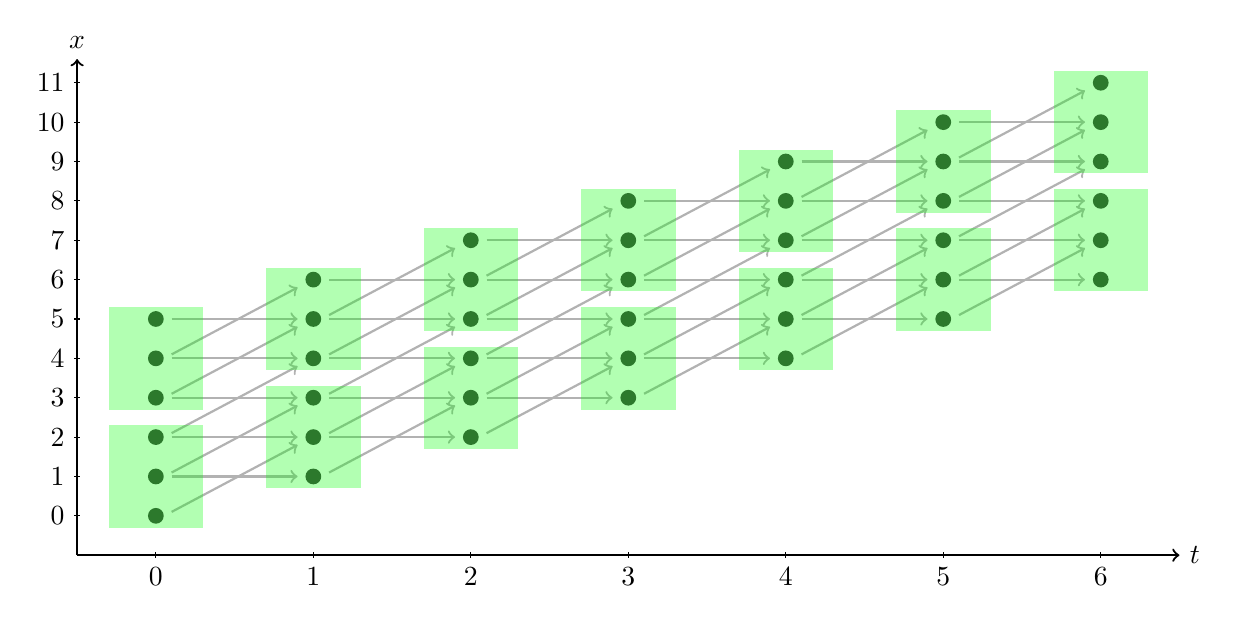
\begin{tikzpicture}
\draw[thick,->] (-1,-.5) -- (13,-.5) node[right]{$t$};
\draw[thick,->] (-1,-.5) -- (-1,5.8) node[above]{$x$};

\foreach \t in {0,1,2,3,4,5,6}
\foreach \x in {0,1,2,3,4,5}
\fill[darkgray] (\t*2,\x/2+\t/2) circle (0.1);

\foreach \t in {0,1,2,3,4,5}
\foreach \x in {1,2,3,4,5}
\draw[thick,->,gray!60] (\t*2+.2,\x/2+\t/2) -- (\t*2+1.8,\x/2+\t/2);

\foreach \t in {0,1,2,3,4,5}
\foreach \x in {0,1,2,3,4}
\draw[thick,->,gray!60] (\t*2+.2,\x/2+\t/2+.05) -- (\t*2+1.8,\x/2+\t/2+.9);

\foreach \t in {0,1,2,3,4,5,6}
\foreach \x in {0,3}
\fill[green,opacity=0.3] (\t*2-.6,\x/2+\t/2-.15) rectangle (\t*2+.6,\x/2+\t/2+1.15);

\foreach \t in {0,1,2,3,4,5,6}
\draw (\t*2,1pt-.5cm) -- (\t*2,-1pt-.5cm) node[anchor=north] {$\t$};
\foreach \x in {0,1,2,3,4,5,6,7,8,9,10,11}
\draw (1pt-1cm,\x/2) -- (-1pt-1cm,\x/2) node[anchor=east] {$\x$};
\end{tikzpicture}
\caption{A skewed iteration space. Dependencies between blocks have not changed, and interchange is \emph{not} valid. (Skewed) tiles included for reference.}
\label{fig:skewed-loops-skewed-space}
\end{figure}

Note that skewing \emph{does not} change the execution order of the loops, nor does it change the structure of the loop nest.

\paragraph{Common sub-expression elimination}
As skewing is merely a substitution of indices and loop bounds, we do not change the expressions.
Since arithmetic on floats is generally non-commutative, we especially wish to avoid changing the structure of expressions, to simplify testing of the code.

In particular, we ensure than skewing is performed \emph{before} CSE occurs, to avoid expansion during skewing.
CSE does not remove the skew, as it is partially applied in the loop header, and partially in the expression (see Figure~\ref{lst:skewing-simple}).


\section{Time-tiling}
\label{sec:time-tiling}
As we noted in the previous section, skewing has not changed the execution order: when applying the tiling transformation, we now have skewed tiles on a skewed iteration space (Figure~\ref{fig:skewed-loops-skewed-space}).
We now need to `straighten' the tiles by aligning the loop bounds.


\subsection{Aligning the loop bounds}
We need to modify the tiling transformation slightly to make the interchange valid.
This was explored in Section~\ref{sec:bg-time-tiling}.
As this alignment was achieved alongside bounding for valid array accesses (detailed in the next section), Figures~\ref{lst:skew-straight} and~\ref{fig:skew-straight} are for illustrative purposes only.

\begin{figure}[!ht]
\begin{lstlisting}
for (int t_blk = t_s; t_blk < t_e; t_blk += t_blk_size)
  for (int t = t_blk; t < min(t_e, t_blk + t_blk_size); t++)
    for (int x_blk = x_s; x_blk < x_e + t_e; x_blk += x_blk_size)
      for (int x = x_blk; x < min(x_e + t_e, x_blk + x_blk_size); x++)
        A[t][(x-t)] = A[t-1][(x-t)-1] + A[t-1][(x-t)+1];
\end{lstlisting}
	\caption{Code which has been tiled following a skewing transformation. This code contains invalid array accesses.}
	\label{lst:skew-straight}
\end{figure}

\begin{figure}[!ht]
	\centering
	\begin{tikzpicture}
	\draw[thick,->] (-1,-.5) -- (13,-.5) node[right]{$t$};
	\draw[thick,->] (-1,-.5) -- (-1,5.8) node[above]{$x$};
	
	\foreach \t in {0,1,2,3,4,5,6}
	\foreach \x in {0,1,2,3,4,5,6,7,8,9,10,11}
	\draw (\t*2,\x/2) node[cross=2.4,red]{};
	
	\foreach \t in {0,1,2,3,4,5,6}
	\foreach \x in {0,1,2,3,4,5}
	\fill[darkgray] (\t*2,\x/2+\t/2) circle (0.1);
	
	\foreach \t in {0,1,2,3,4,5}
	\foreach \x in {1,2,3,4,5}
	\draw[thick,->,darkgray!60] (\t*2+.2,\x/2+\t/2) -- (\t*2+1.8,\x/2+\t/2);
	
	\foreach \t in {0,1,2,3,4,5}
	\foreach \x in {0,1,2,3,4}
	\draw[thick,->,darkgray!60] (\t*2+.2,\x/2+\t/2+.05) -- (\t*2+1.8,\x/2+\t/2+.9);
	
	\foreach \t in {0,1,2,3,4,5,6}
	\foreach \x in {0,3,6,9}
	\fill[green,opacity=0.3] (\t*2-.6,\x/2-.15) rectangle (\t*2+.6,\x/2+1.15);
	
	\foreach \t in {0,1,2,3,4,5,6}
	\draw (\t*2,1pt-.5cm) -- (\t*2,-1pt-.5cm) node[anchor=north] {$\t$};
	\foreach \x in {0,1,2,3,4,5,6,7,8,9,10,11}
	\draw (1pt-1cm,\x/2) -- (-1pt-1cm,\x/2) node[anchor=east] {$\x$};
	\end{tikzpicture}
	\caption{Straightened tiles on a skewed iteration space. Invalid array accesses indicated by crosses.}
	\label{fig:skew-straight}
\end{figure}

\subsection{Making the tiling transformation valid}
% TODO: elaborate: challenges, specific details
Having straightened the tiles (as in Figure~\ref{fig:dependence-skew}),

% Parallelism troubles leading to the Visitor
\paragraph{Parallelism}

\subsection{Testing}

\subsection{User-defined blockshapes}

\subsection{Auto-tuning}

\section{Further work}
The implementation work that remains can be divided into several tasks:

\begin{description}
	\item[Time-tiling] This is mostly complete. Some outstanding items:
	\begin{itemize}
		\item Removal of `empty' blocks -- trivial; does not affect correctness but might produce speedup\footnote{CLooG does it, but one has difficulty imagining that there will indeed be a noticeable speedup}
		\item Making this work with time buffering -- some reasoning about skewing factor required
		\item Test cases -- more can be added
		\item Removal of test cases assuming a remainder loop structure
		\item Verification that a given skewing factor is valid -- this should be very easy as Devito knows all about the stencil
	\end{itemize}

	\item[DSE aggressive mode] Currently, no reason to suppose that this cannot work with \texttt{min}-bounded instead of remainder loops. Need to prove/disprove this, and make it work. Revert to remainder loops if necessary. In particular, we must examine the references made to certain variables.\footnote{Of particular interest are \texttt{blockshape} (the tile size) and dimension extents (e.g.~symbolic extent vs offsets).}

	\item[Sparse loop interpolation] Gather more context and understanding of the problem will be important for reasoning about how this affects time-tiling. Ideally, eventually a proof of what it does/why it does not.

	\item[Detection of when to apply skewing and calculation of the skewing factor] Whether time-tiling is an appropriate optimisation, for a given stencil. Entirely beyond the scope of this work.
\end{description}
